\chapter{User Guide}

In this guide, we will walk you through how to use the Emmy emulator, a \glsdesc{gb} and \glsdesc{gbc} emulator for the browser.

\section{Disclaimer}

Emmy is not affiliated with Nintendo in any way. You are responsible for obtaining copies of the \glspl{rom} you wish to play yourself, and must ensure you are allowed to have these \glspl{rom}. Open source \glspl{rom} are available online, on websites like Retro Veteran\ftnt{https://www.retroveteran.com/category/nintendo-game-boy-color/}. We do not condone the usage of illegally obtained \glspl{rom}.

One feature of the emulator involves using boot \glspl{rom} for the console. These cannot be distributed by Emmy, and must be obtained legally to be used. These can be found and downloaded online. They are not necessary for the usage of the emulator. Open source versions of the boot \glspl{rom} can be found online.


\section{Playing games on Emmy}

First, open the emulator from your browser -- a hosted version is available at \url{https://emmy-gbc.vercel.app/}. You will get to the Emmy emulator (see figure \ref{fig:emmy-startup-screen}).

\begin{figure}[h]
    \centering
    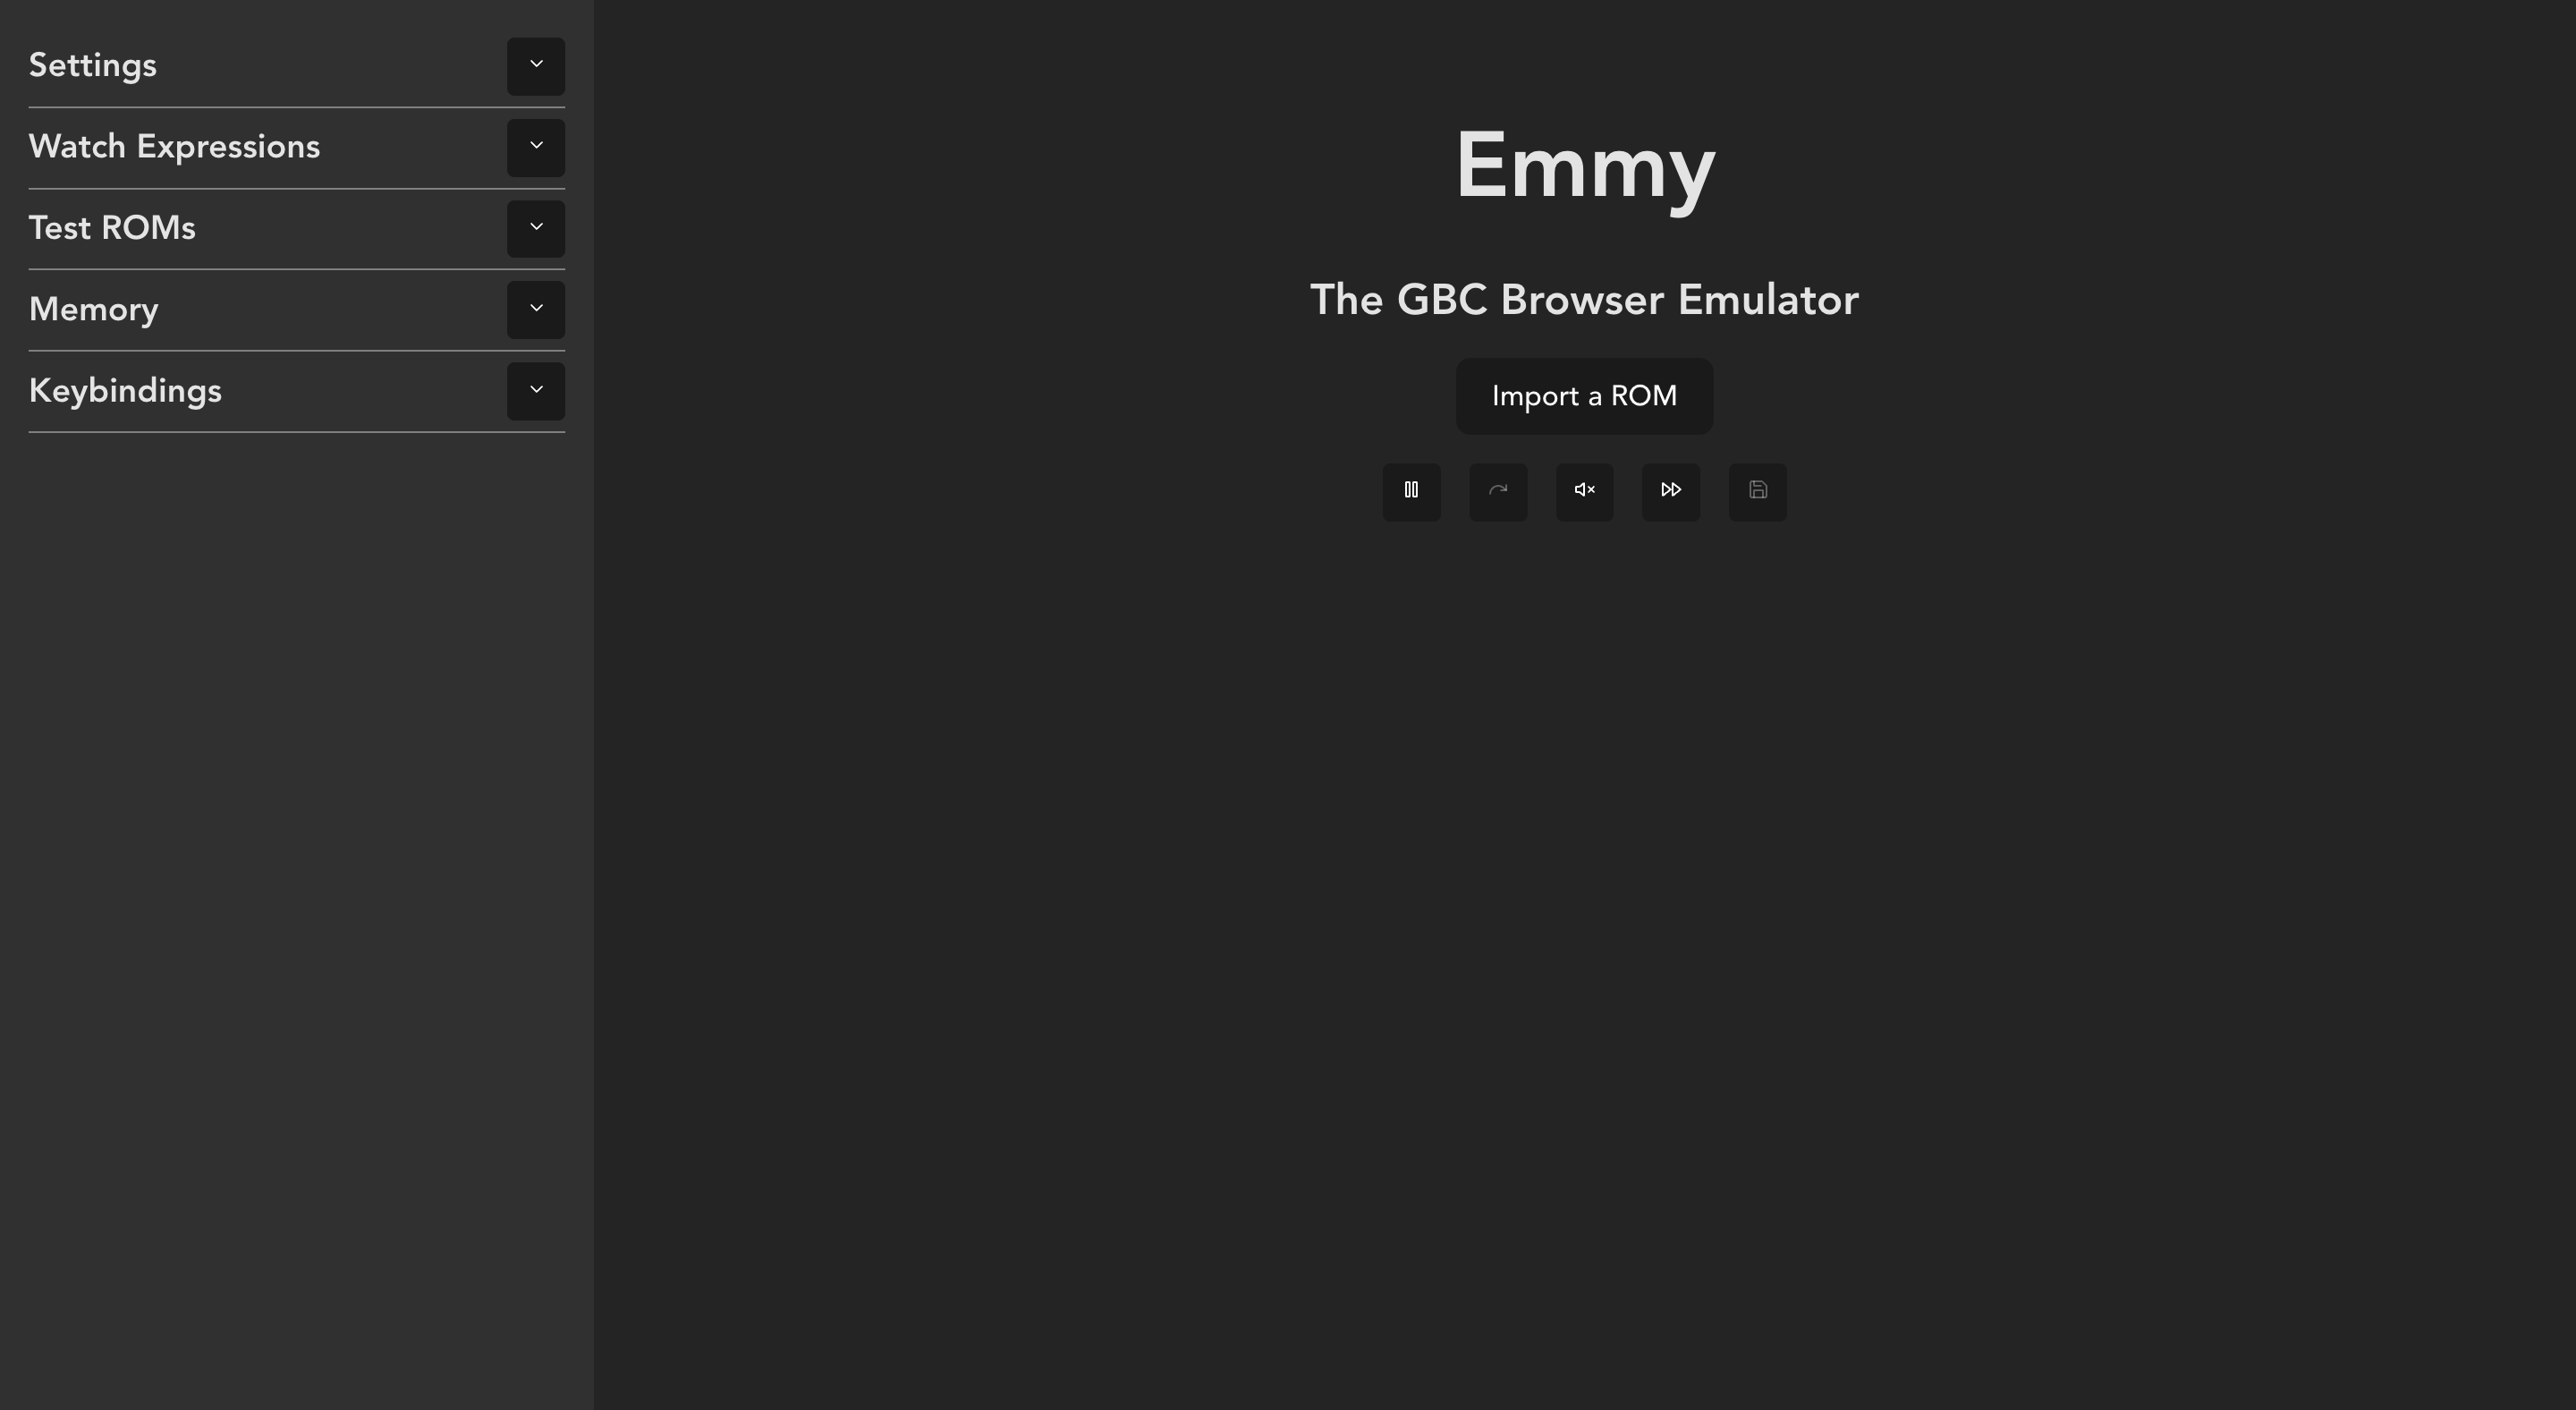
\includegraphics[width=12cm]{images/emmy-startup-screen}\\
    \caption{Start screen of Emmy}
    \label{fig:emmy-startup-screen}
\end{figure}

The interface is divided into two parts:

\begin{compactitem}
	\item The main area, on the right. This is where the console's screen will appear. It has a extra buttons, that we will talk about later.
	\item The sidebar, on the left. This is where all of the settings of the emulator are. All submenus can be opened and closed.
\end{compactitem}


Press the ``Import a ROM'' button, to select the \gls{rom} you wish to use. A file picker dialogue should open -- select the \gls{rom}, and start playing! The game should directly load into the emulator.

\section{Settings}

The behaviour of Emmy can be customised to your needs. In the main area, you can find buttons to freeze the play-through, or resume it. You can also decide to enable or disable the game's sound, and speed up the emulation, making it go three times as fast. If the game supports save files, press the ``Save'' button to save the current state of the game. The next time you open the \gls{rom}, your save will automatically be loaded.

In the sidebar, you will find more settings to customise the emulator (see figure \ref{fig:emmy-settings}).

\begin{figure}[h]
    \centering
    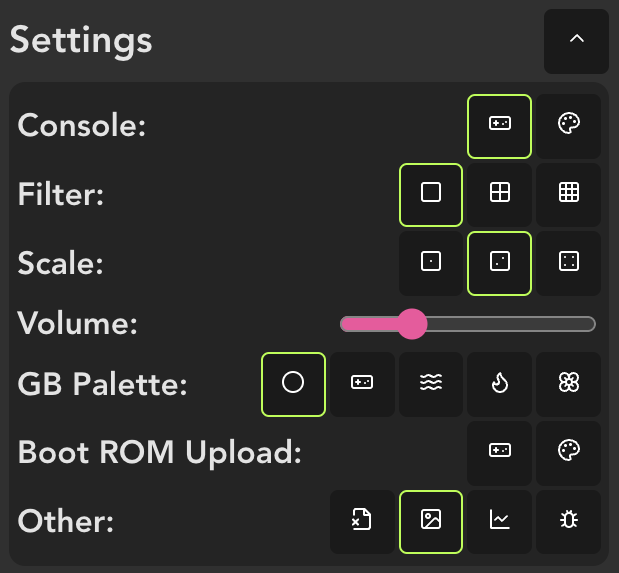
\includegraphics[width=5cm]{images/emmy-settings}\\
    \caption{Settings of Emmy}
    \label{fig:emmy-settings}
\end{figure}

From top to bottom, these settings are:

\begin{compactitem}
	\item The emulated console. This may either be the classic \glsdesc{gb}, or the \glsdesc{gbc}.
	\item The upscaling filter chosen. This option modifies the output of the screen. The first option leaves it as it is, without altering it. The two other options, Scale2x and Scale4x\ftnt{https://www.scale2x.it/}, allow upscaling the image, by adding more details to it, increasing its resolution by two and four respectively.
	\item The scale at which the screen is displayed. This allows increasing the size of the screen -- not its resolution!
	\item The volume at which the emulator outputs sound (if audio is enabled).
	\item The palette used for the \glsdesc{gb}. By default, it will use shades of grey. Options include the classic green hues, a blue palette, a darker red palette, and a flowery pink theme.
	\item Two buttons to upload the boot \gls{rom} of the emulator. This isn't needed to play, but can be nice if you want the original startup screen.
	\item A set of miscellaneous settings, including:
	\begin{compactitem}
		\item If the boot \gls{rom} is enabled. For this to work, you must have first uploaded a boot \gls{rom} for the current console.
		\item Enabling frame blending, meaning frames are blended together. This may cause some slight visual artefacts when the scene is moving around.
		\item Displaying the current performance of the emulator.
		\item Displaying the tileset and tile data of the emulator. This is intended for debug purposes.
	\end{compactitem}
\end{compactitem}

\section{Keybindings}

Emmy comes with default keybindings for the controls, that are common in other emulators (see figure \ref{fig:default-keybindings}). 

\begin{figure}[h]
    \centering
    \begin{tabular}{|l|l|}
    \hline
    \textbf{Game Boy Button} & \textbf{Default Key} \\ \hline
    Directional arrows & Directional arrows \\ \hline
    A & Z \\ \hline
    B & X \\ \hline
    Start & Enter \\ \hline
    Select & Backspace \\ \hline
    \end{tabular}
    \caption{Default keybindings of Emmy}
    \label{fig:default-keybindings}
\end{figure}

These can also be customised, in the ``Keybindings'' submenu (see figure \ref{fig:keybindings}). To change a keybinding, click on the button you want to remap, and the press the key you want to bind to it. Press enter to confirm, and delete to cancel.

\begin{figure}[h]
    \centering
    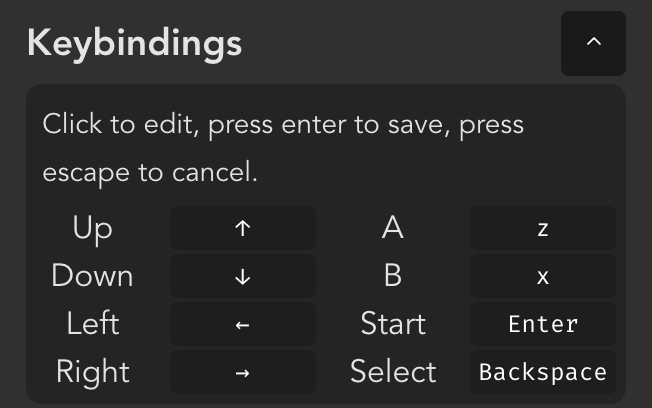
\includegraphics[width=5cm]{images/keybindings}\\
    \caption{Keybindings menu}
    \label{fig:keybindings}
\end{figure}

\section{Debugging}

Emmy also provides a set of debugging tools - if you are a retro game developer, an emulator developer or want to study \glsdesc{gb} \glspl{rom}, these tools will be of great help to you.

First, in the sidebar there is a ``Watch Expressions'' submenu (see figure \ref{fig:watch-expressions}). It allows writing expressions and seeing their output directly from the UI. The syntax is the JavaScript syntax. The emulator is defined as the variable \texttt{gbc}. To access any data on the emulator, refer yourself to the project's code, available at \url{https://github.com/N1ark/gbc-emulator}. The emulator is in the \texttt{src/emulator} folder.

\begin{figure}[h]
    \centering
    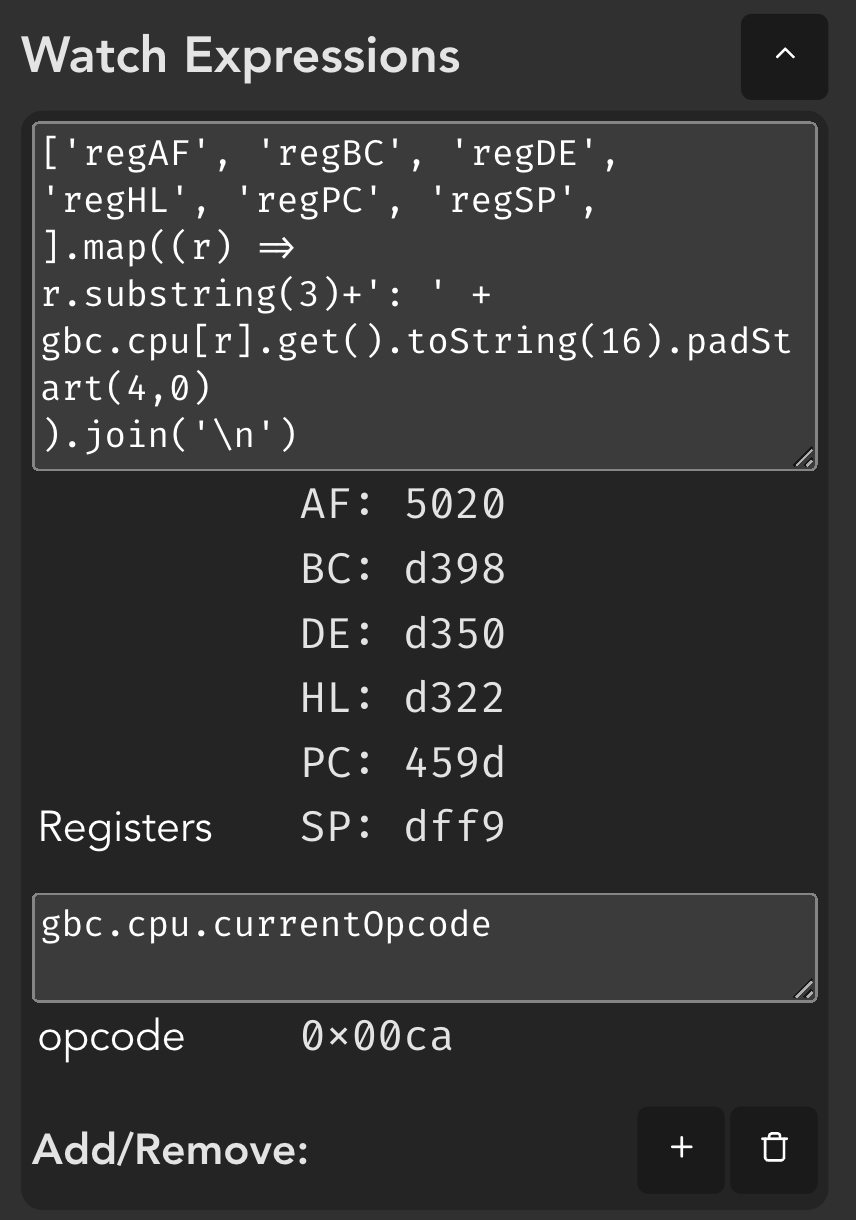
\includegraphics[width=5cm]{images/watch-expressions}\\
    \caption{Settings of Emmy}
    \label{fig:watch-expressions}
\end{figure}

For instance, to access the \texttt{DIV} register of the timer, use the expression \texttt{gbc.system.timer.divider}. By default, number are output in hexadecimal. If you want to see the number in a decimal format, format it into a string: \texttt{num.toString(10)}. You can add and remove as many watch expressions as you want! If one of them is not valid, the message ``\texttt{Error}'' will appear.

The emulator  also comes with a builtin set of test \glspl{rom}, to test the emulator live (see figure \ref{fig:test-roms}). This allows you to easily see how accurate it is, and what tests the emulator passes and fails - this is very useful if you are working on the emulator's code, to ensure you are not breaking anything as you modify it. You can select the set of tests you wish to run, and there is also a button to select or unselect everything.

\begin{figure}[h]
    \centering
    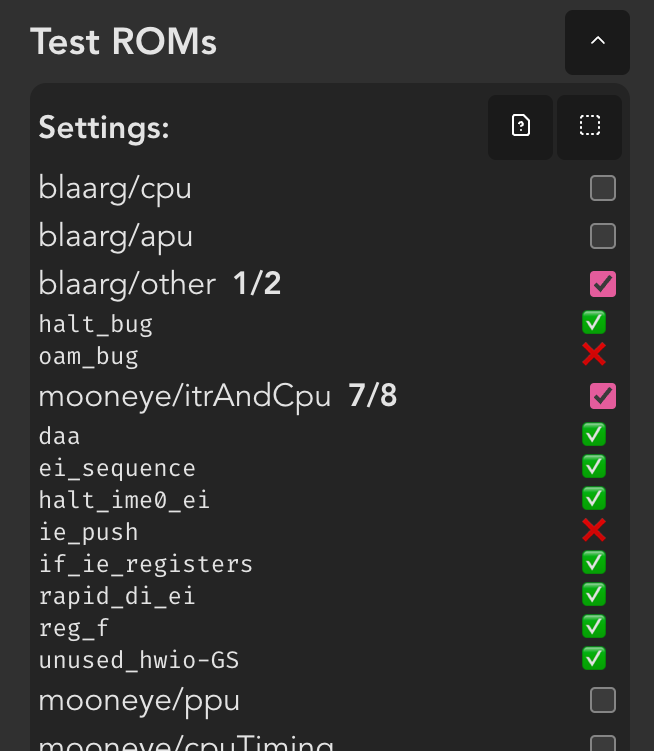
\includegraphics[width=5cm]{images/test-roms}\\
    \caption{Automated test ROMs}
    \label{fig:test-roms}
\end{figure}

To inspect the behaviour of the emulator in detail, the emulator can be paused, and ticked instruction by instruction by pressing the ``Step'' button in the main area. This allows you to see what each instruction does, which is very helpful when a bug arises.

Finally, a memory inspection tool is available, to see the data contained in all of memory. To see it, open the ``Memory'' submenu (see figure \ref{fig:memory-inspect}). It will display every single accessible byte of memory, from \texttt{0x0000} to \texttt{0xFFFF}. If you are only interested in a part of memory, an offset can be input (for instance, if you only want to see the data from \texttt{0xFF00} to \texttt{0xFFFF}).

\begin{figure}[h]
    \centering
    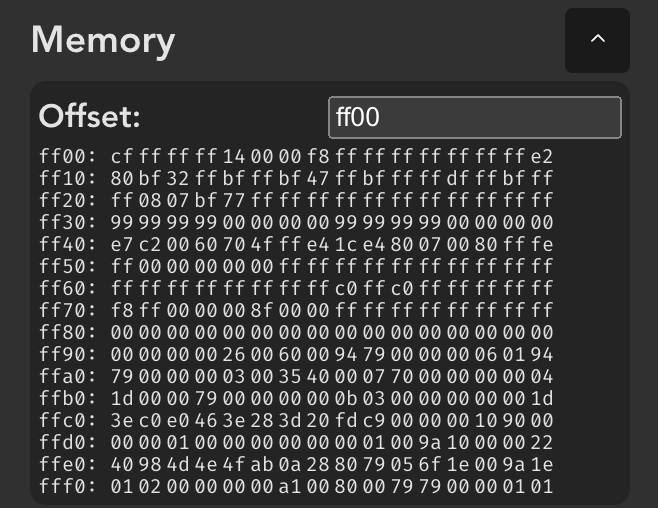
\includegraphics[width=5cm]{images/memory-inspect}\\
    \caption{Memory inspection tool}
    \label{fig:memory-inspect}
\end{figure}